\chapter{Computer Experiments} \label{ch:computer_experiments}
This section describes the setup and configuration of the computational experiments conducted in this study, and the accompanied results. Two types of statistical models, \acrshort{convlstm} and \acrshort{ar}-model are trained and evaluated on a unseen portion of the dataset. 

\section{Hardware} \label{sec:hardware}
%How to deal with big datasets that will easily eat up you memory? ``Big data'' involve processing large amounts of data that does not fit into memory. Processing substantial amounts of data require expert knowledge about distributed systems and analysing for system bottlenecks.  %Although theoretically fascinating it remains to see if \acrshort{convlstm} provide a clear practical advantage over the autoregressive models.
%Conducting experiments on big datasets require external computational resources.  
The experiments are conducted on a 
%This study had access to a 
DGX-2 system consisting of 16 NVIDIA Tesla V100 GPUs, each of 32Gb local memory and 1.5Tb shared memory. %The resources was available through the \acrfull{ex3} project hosted at Simula. 
This study was awarded access 1 GPU and 1024G part of the memory. The data is stored on a \acrfull{rdma} accessed over Infiniband. \textit{The best choice of collective implementation depends upon the number and kind of GPUs, and the network interconnect in the cluster.} \textbf{kopiert derfor kursiv--skal skrives om} %The hardware sets the limitations for efficiency of pipelines and training procedure. 
%\textit{NVIDIA V100 GPU -- The eX3 infrastructure includes a DGX-2 system consisting of 16 NVIDIA Tesla V100 GPUs, allowing simultaneous communication between all eight GPU pairs at 300 GBps through the 12 integrated NVSwitches. This gives a theoretical system-wide system bi-directional  bandwidth of 2.4 TBps. All GPUs have 32 GB of local memory (total of 512 GB) and share a 1.5 TB main memory. The total system has 81,920 CUDA cores, and 10,240 Tensor cores delivering 2 Petaflops of tensor performance. The peak performance in double precision is 125 Teraflops.}

The DGX-2 system is designed for a high level concurrency and scheduling workers competing for system resources. %Working on such a monstrosity pose additional challenges related to porting existing code and virtual environments, developing and debugging code. To eventually end up with an%a achieved 
%acceptable level of efficiency and reliability. \textbf{må de siteres? (\cite{ex3docs} and \cite{ex3homepage}).} 

\begin{table}[ht]
    \centering
    \begin{tabular}{c|c}
        Device &  Type  \\ \hline
        GPU & Tesla V100-SXM3-32GB \\
        CPU & DualProcessor AMD Epyc7601 (SMT2) w/2TB ram and 4TB NVMe 
    \end{tabular}
    \caption{Hardware specifications for our testing environment on \acrshort{ex3}. Operating system is Ubuntu 18.04.4.}
    \label{tab:hardware_ex3}
\end{table}

\section{Framework} \label{sec:framework}
\textbf{Make sure this section contains what you intend to say about the software.}
Mention 
\begin{enumerate}
    \item convlstm is implemented using tensorflow version 2.
    \item ar models are trained and evaluated used self implemented modules available in this project repository 
    This is to ensure that the method utilize the analytical solution to the least squares problems, and not a numerical approximation, developed to cope with non invertable matrices.
\end{enumerate}
%The tensorflow keras API simplifies many aspects of building and executing machine learning models. Its implementation and distribution system aware. This makes the code more versatile, it can easily be ported to other system without many adjustments. 

%This is not the case for the \acrshort{ar}-model and they prove to be more time consuming. \textbf{The task is performed over the entire grid,  .... legg til bedre overgang} Distributed programming involves splitting the data into many tasks. These tasks are then executed in parallel by workers also known as threads. Parallel programming is necessary to take advantage of all the cores on a cluster to accelerate computational science. 

Complex computations will cause memory growth, dependant on how many intermediate computations it needs to store. This is the case for \acrshort{convlstm}. To speed up the development process the software is developed on a subset of \acrshort{ecc}. Small adjustments needs to be made, running experiments on the entire data. For instance threads deadlock when extracting large amounts of data. This is a precautionary measure to avoid overloading the system. \textbf{Possible to develop code to do Hyperparameter tuning based on }

For a more detailed description please see the project repository described in Section \ref{sec:structure_and_implementations}.

\section{Model Setup and Evaluation}
The following sections contain the configurations of the models compiled for this study along with descriptions of hyperparameters. A hyperparameter is a parameter set before the training starts, as mentioned in Section X. A model is compiled based on a choice of hyperparameters. In the search for the best model configuration, different combinations of hyperparameters are tested. This is done manually to begin with since the choice of architecture can easily overload the system memory resources.
%\textbf{The architecture is dependant on the problem, but also the memory resources.}

%It is possible since \acrshort{ar}-models have a small search space. The \acrshort{convlstm} models have a large search space. 
As a starting point for the \acrshort{convlstm} is the set of architectures provided by \citeauthor{SunAirLSTM} (\citeyear{SunAirLSTM}) described in Section \ref{sec:related_work}. For the \acrshort{ar}-models it follows the pricipal of starting with the simplest model possible and increasing the complexity from there. Stopping at architectures where increased complexity don't increase the performance? Know stategies are using spaced sampling, attempting lags of 1, 2, 5, 10. The second is naturally to further investigate regons of lags showing the most promise. 
%on a similar problem, air quality forecasting problem was executed. \citepaper{chollet2015kerastuner} provide suitable software for the automatic hyperparameter tuning. 
%\textbf{Man kjører eksperimenter på mange modeller ved å bruke traning og validations dataset. The choice of model is based on this data basis and then it performance is tested on the test dataset.} 

The partitioning into training and test data is inherited from the model. Since the AR-modelling is done based on a analytical solution there is no need for a validation dataset. Both model are tested on 2014 to 2018. For \acrshort{ar}-models this is trained on 2004 to 2013 and the \acrshort{convlstm} trained on  2004 to 2011 and validated on  2012 to 2013. The test period was chosen based on the assumption that the latest period is most representabel for the climate in the near future.

%Inherited from the problem the \acrshort{ar}-models dataset is split into two portions, training and test. This is sufficient, since there exist an analytical solution to this problem, as mentioned in Section \ref{sec:ARmodels}. 
%For the \acrshort{convlstm} there is no analytical solution, there is a numerical solution, this introduce the need for a validation dataset. 
Another minor differences for the datasets prepared for the \acrshort{ar} and the \acrshort{convlstm}-models. The order of the \acrshort{ar}-model determine the length of the training sequence. All samples with gaps in the requested sequence is disregarded causing a reduction in the data basis for a particular model. For the \acrshort{convlstm} these gaps are filled with a out-of-sample value, $c=1.5$.


\subsection{Autoregressive models}
%\textbf{Move first two paragraphs to discussion..?}
\textbf{Bedre å dra inn software her?}
The python package ``sciclouds'' provide a self implemented version of \acrshort{ar}-models, using the analytical solution to the least squares problem derived in Section \ref{sec:ARmodels}. %This has major improvement possibilities. 

A set of models are compiled by varying components like scaling the predictors, transforming the target, the inclusion of intercept, order of the models and environmental variables. A summary of the calibrated models are provided in Table \ref{tab:ar_model_config}. Keep in mind that one AR-model is the combination of 13041 individual regression models.  

%Time consuming task because of the high number of matrix inversions. A double for loop over this takes to long and \textbf{mention the version of paralelization used on this problem}.

\subsubsection{Feature Scaling} \label{sec:scaling_predictors}
%Feature standardization makes the values of each feature in the data have zero-mean 

Feature scaling is used to standardise the predictor variables.
%By subtraecting the mean and dividing by the variance, t
Applying Equation \ref{eq:scaling_data} to the predictors reshapes the distribution toward a standard normal distribution with zero mean and unit variance. 
%Data transformation can be beneficially in an attempt 
Tranformation offers an additional benefit of increased numerical stability. %When applied the predictors is transformed according to the following Equation \ref{eq:scaling_data}. 
The feature scaling is applied after the partition into training and test dataset, the mean and standard deviation is computed based on the training set. In this manner the trained model avoids sneak peaking at the test data, resulting in a unrepresentative measure on performance.
\begin{equation} \label{eq:scaling_data}
    \mathbf{x} = \frac{\mathbf{x} - \bar{\mathbf{x}}}{\sigma_{\mathbf{x}}}
\end{equation}
where $\bar{\mathbf{x}}$ is the average and $\sigma$ is the standard deviation. The model is trained to find relations in transformed data. Before making predictions based on test data it need to be transformed, using the mean and standard deviation from the training sample.

\subsubsection{Transforming target} \label{sec:transforming_target}
A trick to avoid prediction unphysical values is fitting against a transformed target. In this study, the target, \acrfull{cfc} ranges from 0 to 1. By applying the inverse sigmoid transformation, see Equation \ref{eq:sigmoid} \textbf{update to inverse sigmoid} the target takes values from the entire real axis $(-\infty, \infty)$. 
The inverse transformation, ordinary sigmoid, transforms the values back to the range [0, 1]. Thereby alleviating predictions of out-of-sample values. The sigmoid function is shown in figure \ref{fig:activation_func_plus}. 
\begin{figure}
    \centering
    \includegraphics[scale=0.45]{Chapter3_Method/figs/activation_functions_and_derivatives.png}
    \caption{Sigmoid function and other activation functions.}
    \label{fig:activation_func_plus}
\end{figure}

\subsubsection{Order \textbf{(update to lag?)} and Environmental variables}
The dataset for a particular model is a combination of the order and whether envoirnmental variables such as $t2m$, $sp$, $q$ and $r$ is included. The eviornmental variables never appear in isolation.
Order the number of time steps of previous cloud cover includes as predictors.% and the inclusion of environmental variables, temperature, surface pressure, specific and relative humidity. 
All model is trained either on the full set of environmental variables or none of them.

\subsubsection{Experimental setup AR-models}
Table \ref{tab:ar_model_config} shows a summary of the \acrshort{ar}-models included in this study. 

\begin{table}[h]
    \centering
    \resizebox{\textwidth}{!}{%
    \begin{tabular}{ccccc}
    \cline{2-5}
     & \textbf{Scaling predictors} & \textbf{Transforming target} & \textbf{Order} & \textbf{Enviornmental variables} \\ \hline
    \multicolumn{1}{c}{\textbf{Model 1}} & \checked & $\times$  & 1 & $\times$ \\ \hline
    \multicolumn{1}{c}{\textbf{Model 2}} & \checked & $\times$  & 0 & \checked   \\ \hline
    \multicolumn{1}{c}{\textbf{Model 3}} & \checked & $\times$  & 1 & \checked  \\ \hline
    \multicolumn{1}{c}{\textbf{Model 4}} & \checked & $\times$  & 2 & \checked  \\ \hline
    \multicolumn{1}{c}{\textbf{Model 5}} & \checked & $\times$  & 3 & \checked  \\ \hline
    \multicolumn{1}{c}{\textbf{Model 6}} & \checked & $\times$  & 4 & \checked  \\ \hline
    \end{tabular}%
    }
    \caption{Configuration of \acrshort{ar}-models. $\times$ denoted not applied, \checked denotes applied \textbf{add bias??} Gi modellen navn basert på configurasjonen $AR_{STEx}$ where x is the order. \textbf{add column of number of parameters and score to avoid extra tables?}}
    \label{tab:ar_model_config}
\end{table}

\subsection{Convolutional LSTM}
\textbf{starter med igjen repetisjon ....}
The formulation of the Air quality forecasting problem presented by  \citeauthor{SunAirLSTM} is similar to the formulation of the cloud fractional cover prediction problem presented in this project. The machine learning experimental setup is adopted from the paper \citepaper{SunAirLSTM}. 
% Endrer på arkitekturen - denne bruker -train - validation - test, en hvis prosentandel a
A lot of architectural decisions (batch size, sequence length, number filterers and number layer) can cause the \acrshort{gpu} to run out of memory. In that case it didn't learn anything. According to \citepaper{ioffe2015batch} Batch Normalization, makes is easier to train models. The feature was added between each layer. Epochs is the number of times the model has seen the entire dataset. The dataset is partitioned into subsets called batches. The batch size is the number of samples a weight update is based on. The sequence length is the \textbf{quite selv explanatory, still need to explain it.. } Number of hidden states .. 

\begin{table}[]
    \centering
    \resizebox{\textwidth}{!}{%
    \begin{tabular}{clcccc}
     & \textbf{Sequence length} & \textbf{batchsize} & \textbf{epochs} & \textbf{MSE} & \textbf{Num Parameters} \\ \hline
    \textbf{Model 1} &  & fdfdf &  &  &  \\ \hline
    \textbf{Model 2} &  & $\checkmark$ &  &  &  \\ \hline
    \textbf{Model 2} &  &  &  &  &  \\ \hline
    \textbf{Model 2} &  &  &  &  &  \\ \hline
    \textbf{Model 2} &  &  &  &  &  \\ \hline
    \textbf{Model 2} &  &  &  &  &  \\ \hline
    \end{tabular}%
    }
    \caption{Configuration of traninable convolutional lstm models. \textbf{r2 er veldig merkelig foreløbig, includere mae?} TODO: Add list of model configurations which actually learn something.}
    \label{tab:convlstm_config}
\end{table}

\textbf{Add drawing of best convolutional lstm model from tikz! Much easier to expain, plus its a nice addition.}


\section{Results}
\textbf{This section presents comparisons from the best convolutional lstm model and the best AR-model. Recall that the Convolutional LSTM model is chosen based on its score of predicting the sequence length and the AR-model is currently evaluated on its performance predicting one step a head. \textbf{Dette er en mismatch som kanskje bør ryddes opp i ..}}

\textbf{Føler det er unødvendig med ekstra tabeller her når du passe så lett sammen med model configurasjons tabellene. Det blir også lettere å tolke om det står sammen.. Hva tenker du..? }

\subsection{Predicting next timestep -- remove or train convlstm model to predict one step}
Currently not made any conv lstm models predicting one step ahead....
%%%% TARGET PREDICITON ERA5
\begin{figure}[ht]
    \centering
    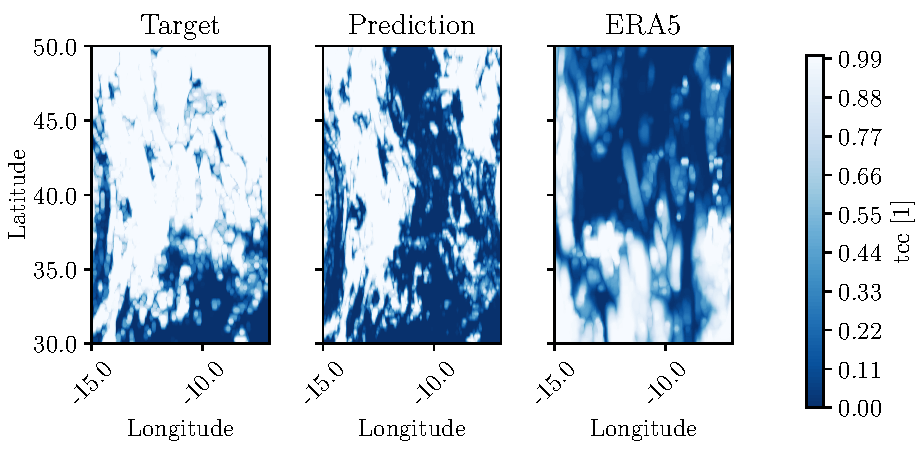
\includegraphics{python_figs/target_prediction_era5_plot_horizonal.pdf}
    \caption{Comparison target, predicted and era5 horizontal cloud fractional cover. Imagine this plot, with a row for each step in the predicted sequence and each column being (AR, Convlstm, target)}
    \label{fig:target_predict_era5_horizontal}
\end{figure}


\subsection{Predicting next 24 hours (or another sequence depend on which models learns this)}
%%%% TARGET PREDICITON ERA5
\begin{figure}[ht]
    \centering
    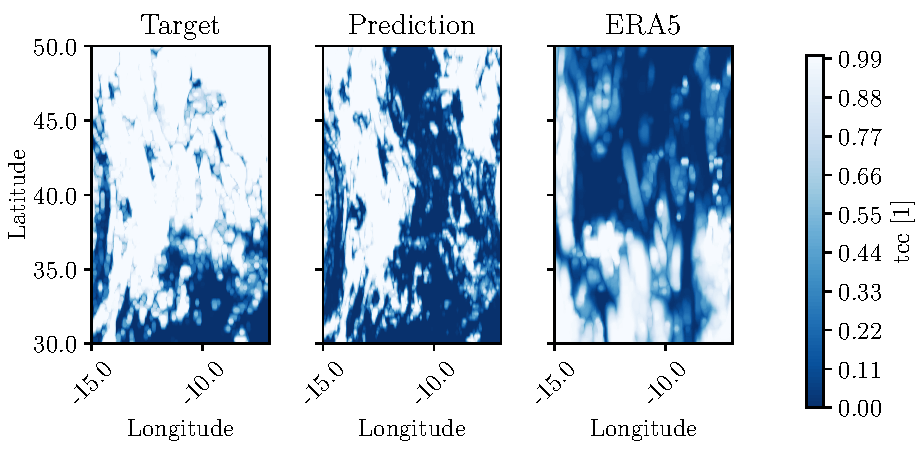
\includegraphics{python_figs/target_prediction_era5_plot_horizonal.pdf}
    \caption{Comparison target, predicted and era5 horizontal cloud fractional cover. Imagine this plot, with a row for each step in the predicted sequence and each column being (AR, Convlstm, target)}
    \label{fig:target_predict_era5_horizontal}
\end{figure}

%\subsection{Autoregressive models}
%%%% TARGET PREDICITON HORIZONTAL
\begin{figure}[ht]
    \centering
    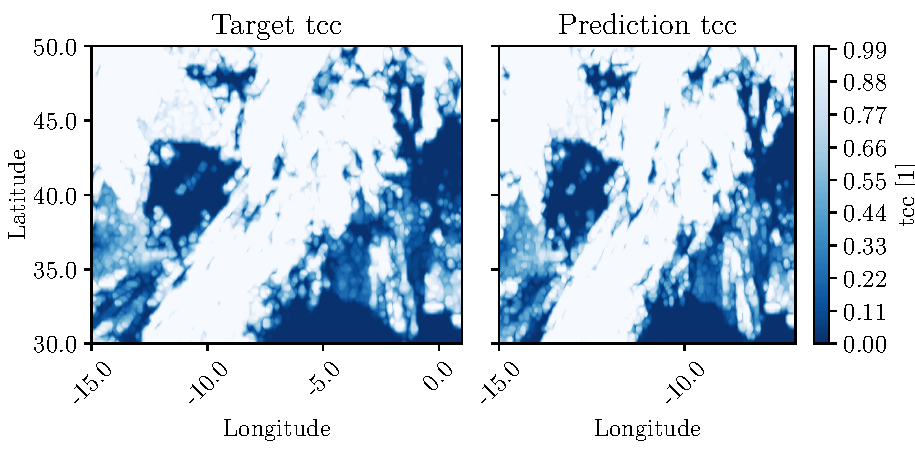
\includegraphics{python_figs/target_prediction_plot_horizonal.pdf}
    \caption{Comparison target and predicted cloud fractional cover.}
    \label{fig:target_predict_horizontal}
\end{figure}

%%%% TARGET PREDICITON HORIZONTAL
\begin{figure}[ht]
    \centering
    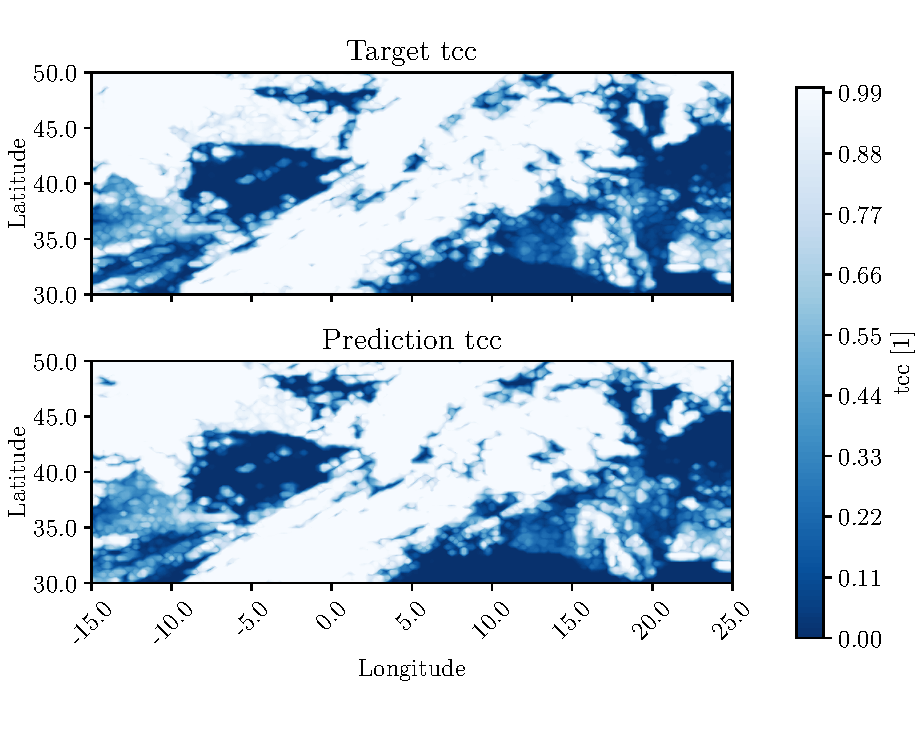
\includegraphics{python_figs/target_prediction_plot_vertical.pdf}
    \caption{Comparison target and predicted vertical cloud fractional cover.}
    \label{fig:target_predict_vertical}
\end{figure}

\section{Practical implications - OUTDATED} \label{sec:practical_implications}
It is necessary to have a understanding of the needs of the end product before conducting large machine learning projects. Answering questions like: What will it be used for and how can it be implemented in useful way?

A major downside of the data driven learning approach is the rigid resolution. A trained model can only be used on similar problems, with the same spatiotemporal resolution. For applications like climate models, output comes in a wide range of different resolutions. Before implementing the finished product in a new model of a different resolution, it would need to be retrained on the resolution of the climate model under development. This process involves both remapping of the dataset and retraining the model at the correct resolution. This is a time consuming process involving finding a new set of hyperparameters suitable for the new resolution. % It essentially means starting over.

Once trained on global climate datasets, machine learning models provide fast results even for complex parameterisation which is what makes them suitable for the application of climate modelling. Most machine learning packages are developed using Python. \acrfull{esm} are implemented in python. Methods for including the trained parameterizations need to be developed.
 
\subsection{Any implications based on the results presented in this chapter.}